\subsection{POMDP}
We face a finite-horizon Partially Observed Markov Decision Process (POMDP), which we define as the tuple $(S,A,O,T,\Omega,R,\gamma,F)$, where:
\begin{itemize}
  \item $S$ is a set of discrete states, $A$ is a set of discrete actions, and $O$ is a set of continuous observations.
  \item $T(s,a,s') = P(s_{t+1} = s | a_t = a, s_t = s)$ is the distribution describing the probability of transitioning from state $s$ to state $s'$ upon taking action $a$.
  \item $\Omega(o,s,a) = P(o_{t+1}=o | a_t = a, s_{t+1} = s)$ is the distribution describing the probability of observing $o$ from state $s$ after taking action $a$.
  \item $R(s,a)$ is the reward signal received when executing action $a$ in state $s$.
  \item $F$ is the deadline to first evaluation.
\end{itemize}

The problem is naturally episodic, where an image presents an episode.
Our goal is to learn the optimal policy $\pi$, which is a mapping from histories (trajectories) $h_{1:t}=((a_1,o_1,r_1)...,(a_t,o_t,r_t))$ to actions $a$.

\subsection{State representations}
For all approaches described later, the state $s \in S$ is fully defined by the time $T$, and the class of the bounding box centered at each location.
We augment the $K$ classes with a ``background'' class, which means that there is no object of interest at a location.
Note that each object in the image is assigned to exactly one location; this is in contrast to many detection models employing random fields, such as~\cite{Torralba2004}.
The number of states is exponential in $N$.

An interesting aspect of our task is that we are dealing with a static image, meaning that nothing changes the underlying state.
Therefore, $T(s,a,s') = \delta_{s, s'}$ where $\delta$ is the Kronecker delta function.
In the usual POMDP setting, the physical state is non-stationary, and a repeated action $a$ may lead to different observations $o$.
In our case, it does not make sense to run the same detection action at a location more than once, and so there is a finite number of actions $\mathcal A$ (not just action types) for us to take in an episode.
This means that $F$ can be set to a finite time $F_{max}$, such that all the possible actions can be taken before termination.
This corresponds to an exhaustive search.

Normally in POMDPs, the history $h$ is unbounded (except by the horizon) and quickly becomes intractably large.
For this reason, POMDP policies are either \emph{memoryless}, meaning that the next action depends only on the last observation, or depend on some internal state representation that is a compression of the trajectory.
A common internal representation is the belief state, $P(s|h_{1:t})$, which can compactly represent everything the program needs to know to make Bayesian-optimal decisions.
If the POMDP is known, then we can convert it with this internal representation to an MDP over belief states, and solve it optimally using MDP techniques.
However, this optimal solution approach is hard to scale to large POMDP problems~\cite{Murphy2000,Ng2000}.
We again note that in our problem, the size of $h_{1:t}$ is always bounded by $\mathcal A$.

We model the internal POMDP state as a graphical model, with nodes for the $N$ locations in the image pyramid, and $N$*$K$ possible observations.
A node $y_{i} \in Y$ is an integer $0 \dots K$, according to the class whose bounding box we believe is centered at location $i$ (background is $0$).
A node $z_{ik} \in Z$ is the real-valued output of a detector of class $k$ at location $i$, signifying classifier confidence.
Two nodes $y_i$ and $z_{ik}$ are connected with weight $w_{k}$, which in a sense represents our confidence in the classifier $c_k$ and also allows us to account for multi-class bias.

The connections between two nodes $y_i$ and $y_j$ are defined by the spatial context feature $d_{ij}$ (represented in~\autoref{fig:dij}) and the weights $w_{y_i,y_j}$.
These weights encode valid geometric configurations of object classes $y_i$ and $y_j$.
\begin{figure}[h!]
  \caption{Figure from~\cite{Desai2009}.}
  \centering
    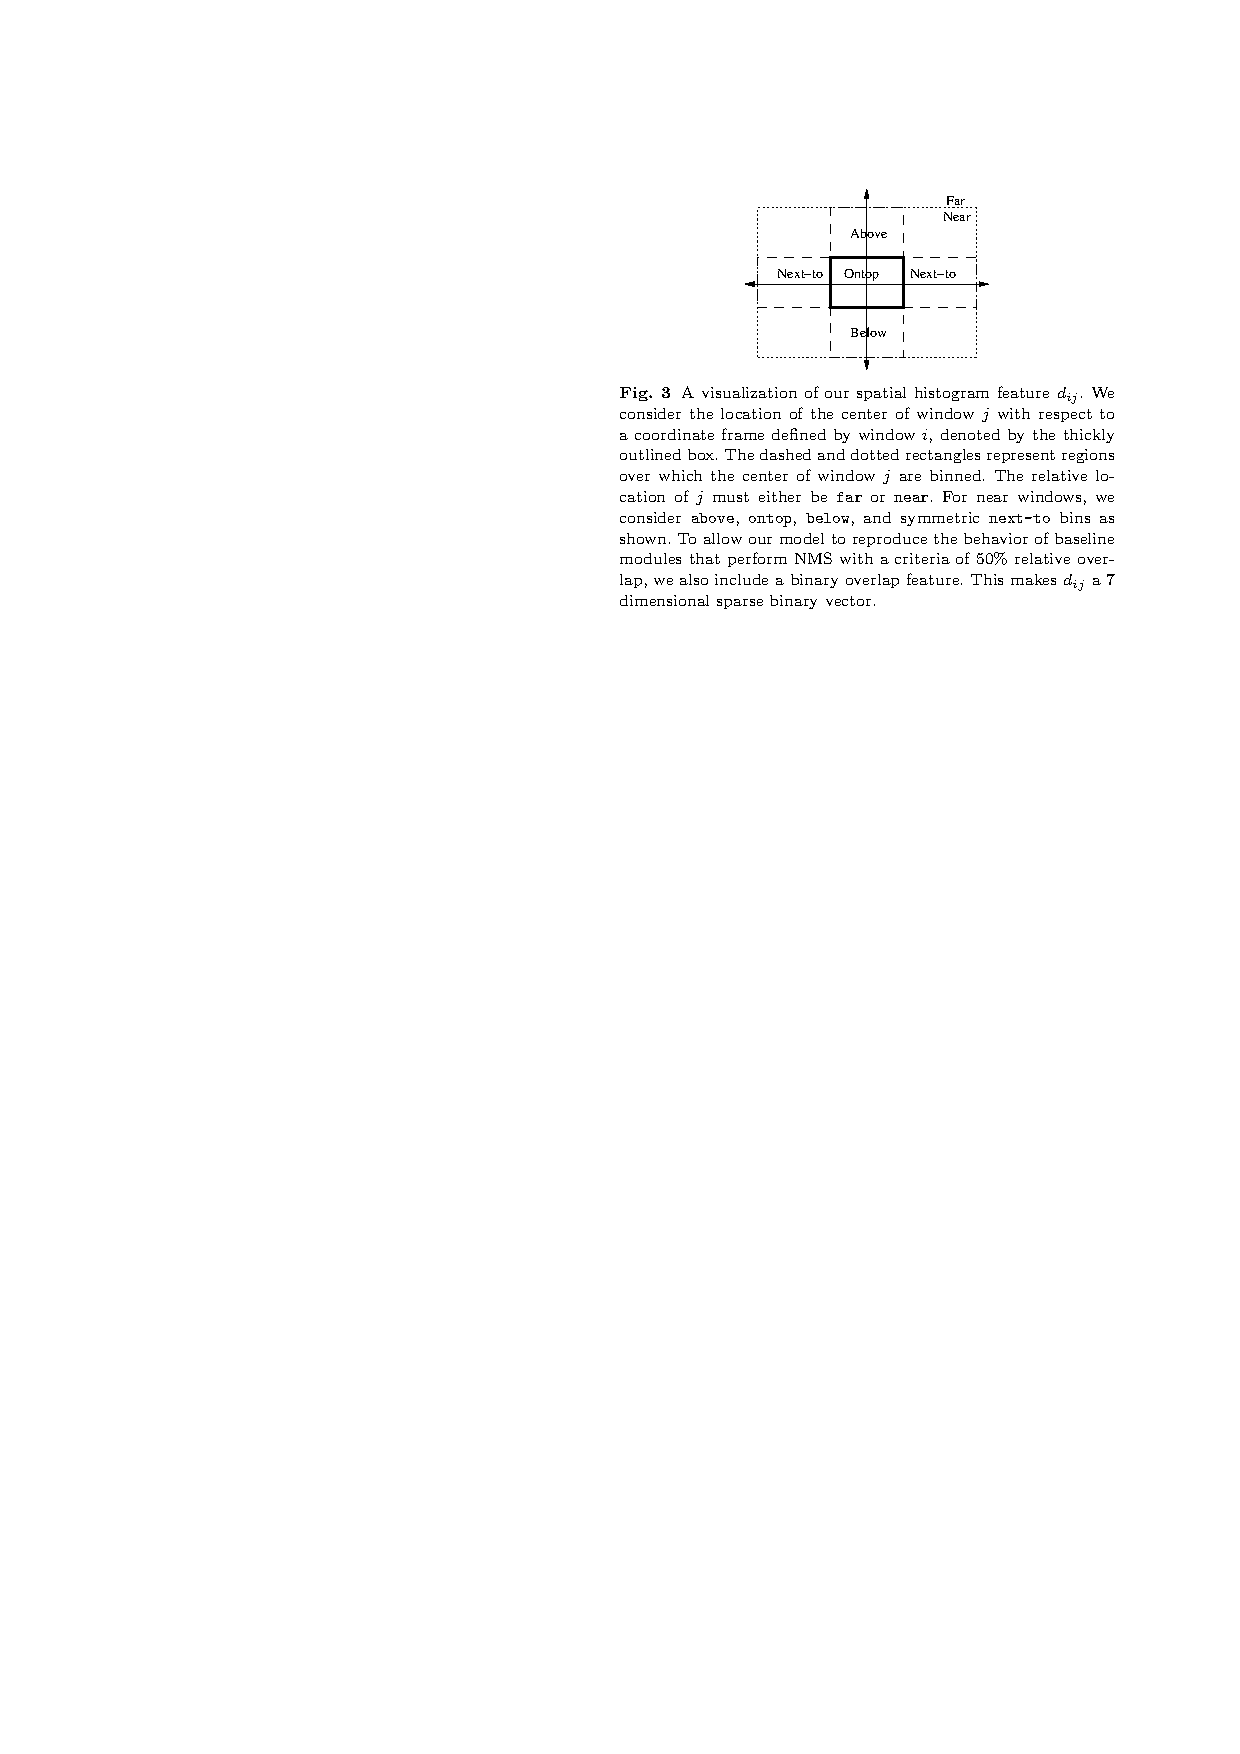
\includegraphics[width=0.7\textwidth]{../figures/dij.pdf}
  \label{fig:dij}
\end{figure}

In this way, we can think of the internal state as a sort of CRF, where $y_i$ are conditioned on the image $X$ through $z_{ik}$.
Crucially, the extra nodes $z_{ik}$ can be unobserved.
This internal state therefore both encodes the full trajectory $h$ (albeit in an orderless way), and provides a model-based probability distribution over $s$.
We note that we do not encode rewards received in the internal representation, and discuss this further in~\autoref{sec:misc}.

This way of modeling the underlying state of the image is similar to the one used in~\cite{Desai2009}.
In fact, we rely on their method of greedy forward search to do inference in the CRF and learn the parameters; inference of the physical state from our belief state is described in~\autoref{sec:rewards}.

\subsection{Actions and Observations} \label{sec:actions}
There are two distinct ways to formulate the action space.

The first defines actions by a choice of location $i$ and detector $c_{k}$, making for $NK$ possibilities.
This action space allows any possible action to be taken at any time, and with the right policy could capture structure of the problem, such as non-maximum suppression and spatial cueing.
The space is considerably large, however, and policies have to be highly complex to be effective.

The second restricts the action space with our domain knowledge of the problem.
For instance, we know there is no point in running the same action twice.
Therefore, we can offer just one action to the agent: ``pick a random unexamined (location,class) pair.''
Of course, the only possible policy then is a random exploration of the space.
To structure the exploration, we can offer action such as ``pick a random class for an unexamined location with the highest entropy of $z_{i}$'' (entropy is discussed in~\autoref{sec:misc}).
We can separate picking the class from picking the location, to for example, obtain a policy of picking an unexplored location of maximum saliency, as determined by some non-state featurization of the image, and picking the class most likely to be in the image, as determined by some other classification output of the image.
Some example policies following this approach are described in~\autoref{sec:example_policies}.

In either case, upon executing an action, the observation $o$ we get back is the confidence of the classifier.
The observation updates the corresponding node $z_{ik}$.
We can propagate this update through the graphical model with an iteration of belief propagation, or alternatively, we can find the MAP assignment to $Y$, given this new information, by running a greedy forward search (details in~\autoref{sec:rewards}).
We can do this at every action, every fixed number of actions, or upon taking a special action.

\subsection{Outputting Detections, Receiving Rewards, and the Deadline} \label{sec:rewards}
$Y$ in our belief state represents the detections, and is conditioned on $Z$.

Recall that we cannot have detections of two different classes at the same location, and that the PASCAL evaluation will penalize all but one detections of the same class at overlapping locations.
For this reason, most detection systems that ``assign content to locations'' like this run a post-processing non-maximum suppression step~\cite{Felzenszwalb2010a}.
In a multi-class setting, it is better to resolve such ambiguities with a principled system to model both inter- and intra-class, and short- and long-range interactions.

Our belief state is modeled after such a system, and we simply run a greedy forward search to maximize the energy of our graphical model to pick our final detections~\cite{Desai2009}.
The energy of the model is given as
\begin{equation}
  S(Y,Z) = \sum_{i,j} w_{y_i,y_j}^T d_{ij} + \sum_{i,k} w_{k} z_{ik}
\end{equation}
In brief, the greedy search starts out with an empty set of detections, and proceeds to pick those $y_i$ that maximize $\Delta S(Y,Z)$.
This method has been shown to be optimal for nearly all images ($\approx98\%$) in the PASCAL set (and compared against Loopy BP and Tree-ReWeighted BP)~\cite{Desai2009}.

The theoretical explanation for this comes from the work on \emph{submodular functions}.
The rough idea is that to maximize functions where adding an element to a large set has less effect than adding an element to a small set, greedy algorithms often have theoretical guarantees of near-optimal performance.
The more pairwise connections are non-positive in the CRF, the more submodular it is.
Since most connections in the image CRF are inhibitory (the CRF mostly performs non-maximum suppression, after all), the theory may apply here.

After every action starting at deadline $F$, $R(s,a)$ is assigned according to the AP of these detections.
The program is not terminated at $F$, but runs to $F_{max}$, which is determined by the time it would take to run every possible detector action once.
Therefore, the reward structure is such that there is a large first reward at $F$, and following rewards at every time step.
It is not clear whether a cost-of-living negative reward should be assigned at each time step; in our toy experiments reported in~\autoref{sec:experiments}, this did not seem to make a difference.
We intend to try both ways on the actual problem.

We express $F$ in units of expected time per action, such that taking action $a$ with time cost $\tau$ advances $T$ by $\tau$.
We determine $\tau$ by averaging the wall clock time of executing $a$; this is done for all $a$ prior to running the POMDP learner.

\subsection{Some Example Policies} \label{sec:example_policies}
We can briefly describe how different detection strategies fit into our framework.
Instead of committing to one strategy, we can define our action space to allow multiple strategies.
We can then find a policy that optimally combines the strategies, perhaps as a function of $T$ and $F$, to maximize the reward under our definitions.

\paragraph{Sliding window, Random, and Saliency-driven}
As described, earlier in the text, our definition of the action space can drive any of these policies.
We first compute a simple, fast self-similarity saliency map for the image (for example, as in~\cite{Alexe2010}).
The internal state is featurized by the location of the current unexamined (picked less than $K$ times) max in the saliency map and the class $k$ of the last action.
The policy could then be to simply sample locations in order of saliency, running all detectors at a location before proceeding to the next.

\paragraph{Class prior or posterior-driven}
On the training set, we compute $K$ canonical object likelihood maps.
We featurize the belief state with the current unexamined (picked less than $1$ time) max of each likelihood map.
Our policy is to run the detector for the class $k$ at the location $i$ with the largest likelihood among these maps.

Of course, with our random field model of the environment, we can compute class posteriors for all locations.
As the policy proceeds, it could start taking belief propagation actions to update the class posteriors and improve the quality of the actions.

\subsection{Unobserved rewards and Augmented MDPs} \label{sec:misc}
Our problem formulation briefly noted an important detail: at test time, the program does not receive rewards.
Therefore, we should not learn a policy that depends on the rewards during execution.
For this reason, there is nothing in our internal state representation that encodes rewards received: the only information is what we currently believe each node $y_i$ to be, and what observations $z_{ik}$ we have made.

We can view the observations $z_i = \{z_{i1}:z_{iK}\}$ as an unnormalized distribution over $y_i$.
Accordingly, we can derive the entropy term $H(z_i)$, which represents our uncertainty in the value of $y_i$.
The idea of adding uncertainty variables to the state space of a decision process is known as Augmented MDPs~\cite{Kwok2004,Roy1999}.
Augmented MDPs have the advantage of increased tractability over corresponding POMDPs, while still retaining the modeling power of allowing uncertainty.
For example, policies can account for the uncertainty in the state through the entropy variables, and direct actions accordingly.
This model has been successfully applied to self-localizing robots~\cite{Roy1999} and to the problem of active sensing in soccer-playing Aibos~\cite{Kwok2004}.

If we model our problem as an Augmented MDP, we will lack one thing: knowledge of the reward function.
Accordingly, we can apply the well-developed array of efficient techniques for model-free reinforcement learning~\cite{Sutton1998}.
Additionally, we can shape the reward function with \emph{a priori} domain knowledge, by, for example, encouraging minimal entropy.

\subsection{Solving the RL problem}
We consider several ways to solve the posed problem.

First, we can attempt to solve the POMDP as a belief-state MDP, computing the state value function for it.
This approach is hard to scale to a problem as large as ours, but efficient methods have been developed for medium-sized problems~\cite{Pineau2006}.

Second, we can solve directly for the $Q(s,a)$ function using reinforcement learning techniques.
For general POMDPs, this seldom works, as the model is likely non-Markovian in $s$.
We consider this approach seriously, because for reasons outlined in ~\autoref{sec:misc}, direct model-free learning could work well for us.
A compromise between this and the first approach was proposed in the $Q_{MDP}$ framework~\cite{Littman1995}, which computes $Q$ as if the environment was Markovian at every future time step past the current one, and so defines $Q(b,a) = \sum_x b(x) Q_{MDP}(x,a)$.
In our toy experiments, we use the technique of Least-squares Policy Iteration~\cite{Lagoudakis2003}, an extension of Least-Squares Temporal Difference learning~\cite{Boyan2002} to model-free learning.
This is an efficient linear method allowing a large number of parameters, and recovering the global maximum of the value function.

Third, we can remember that the ultimate goal is to find the best policy, and search for it directly, forgetting about standard indirect approaches of policy evaluation.
Direct policy search is motivated by indirect approaches' several problems when applied to POMDPs:
\begin{itemize}
  \item $Q$ may be unstable due to non-Markovian $s$; 
  \item function approximation may make it hard for reinforcement learning to converge to a stable policy;
  \item stochastic policies may be better suited than deterministic ones to POMDPs.
\end{itemize}

Direct policy search does not suffer from these problems, but of course has the additional problem of how to parametrize and learn the policy effectively~\cite{Murphy2000,Hauskrecht2000}.
An effective way to represent a policy is as a Finite State Machine~\cite{Hansen1998}, which can lead to efficient search solutions.
The PEGASUS framework samples trajectories most efficiently, allowing fast search through a huge space~\cite{Ng2000}.
A series of reports on the GPOMDP algorithm extend the ideas began in Williams's REINFORCE algorithm~\cite{Williams1992} for policy gradient ascent and review much of the relevant literature~\cite{Baxter1999,Baxter1999a}.
Lastly, the problem of searching for the best policy can be treated at its most basic, as a coordinate ascent problem~\cite{Kohl2004}.

In our opinion, direct policy search is most suitable for general POMDP problems, as it minimizes the assumptions made about the belief state, and at least directly ensures that the policy is improved at each iteration of learning (value function learning does not guarantee this).
However, the special structure of our POMDP, and the possibility of a reasonable representation as an Augmented MDP, leads us to at least try a reinforcement learning approach to our task.
We describe initial experiments to this end in~\autoref{sec:toy_experiments}.